\documentclass[mathserif]{beamer}
\usepackage{mathtools}
\usepackage{amssymb}
\usepackage{bm}
\usepackage{graphicx}
\usetheme{Copenhagen}

\begin{document}
	\title[Analyzing Stochastic Time-Series Data]{Techniques for Analyzing Stochastic Time-Series Data}
	\author[Castleberry \and Oubre \and Yu]{Dennis Castleberry \and Brandon Oubre \and Haikou Yu}
	\date{\today}
	\frame{\titlepage}
	
	\section{Project Overview}



	\frame{ \frametitle{Project Overview}
		\begin{itemize}
			\item Test a variety of different classifiers on different data sets.
			\item Can we improve classification accuracy of time-series data by adding attributes to current data from previous data?
			\item For example, does informing a classifier of the class of the previous \(n\) entries improve prediction accuracy for the current observation?
			\item How far back should we look and what information should we include?
		\end{itemize}
	}

	% Time series, multivariate, stochastic
	% Our task is prediction of the next time series value: given all the time-dependent data up to
	% this point, we want to know the value of some class for the next iteration/time.
	% E.g. ..

	
	\section{Background}
	\subsection{Naive Bayes}
	\subsubsection{Overview}
	\frame{ \frametitle{The Naive Bayes Classifier}
		\begin{itemize}
			\item Reduce classification to probability. What is \(P(class | attribute1, attribute2, ..., attributeN)\).
			\item Assumes that each attribute is independent of the others. (Hence the ``Naive'' nickname.)
			\item For example, let's consider if a car is stolen using \(P(stolen | Color, Type)\). Naive Bayes will assume \(color=red\) and \(type=sportscar\) to be independent.
			\item Naive Bayes is not sensitive to irrelevant attributes, since the probabilities of such attributes will be similar for all classes.
			\item Naive Bayes is quick to train, as it requires only one pass-though of the training data.
		\end{itemize}
	}
	
	\subsubsection{Example}
	\frame{ \frametitle{Naive Bayes in Action}
		\begin{center} 
			\textbf{Training Data} \\
			\begin{tabular}{c | c | c || c}
				\textbf{Over 170cm} & \textbf{Eye Color} & \textbf{Hair Length} & \(\boxed{\textbf{Sex}}\) \\ \hline \hline
				No & Blue & Short & Male \\ \hline
				Yes & Brown & Long & Female \\ \hline
				No & Blue & Long & Female \\ \hline
				Yes & Brown & Short & Male \\ \hline
				Yes & Brown & Short & Female \\
			\end{tabular}  \\
			\small{Only discrete values shown, but we can still interpret real data using normal distributions!}
		\end{center}
			Suppose we are given an unseen data point \(\langle No, Blue, Short \rangle\). What should we classify it as?
	}
	
	\frame{ \frametitle{Naive Bayes in Action}
		\begin{tabular}{l}
		\(P(Male|No,Blue,Short)\) \\
		\(=\dfrac{P(No,Blue,Short|Male) P(Male)}{P(No,Blue,Short)}\) \\
		\(= \alpha P(Male)\bm{P(No|Male)P(Blue|Male)P(Short|Male)}\) \\
		\(=\alpha \times \frac{2}{5} \times \frac{1}{2} \times \frac{1}{2} \times \frac{2}{2} = \boxed{0.1\alpha}\) \\ \\
		\hline \\
		\(P(Female|No,Blue,Short)\) \\
		\(=\alpha P(Female)P(No|Female)P(Blue|Female)P(Short|Female)\) \\
		\(= \alpha \times \frac{3}{5} \times \frac{1}{3} \times \frac{1}{3} \times \frac{1}{3} = \boxed{0.0\overline{2}\alpha}\) \\
		\end{tabular} \\
		\vspace{10px}
		Since \(P(Male|Data) > P(Female|Data)\), we classify the unseen point as Male. For multiple classes, just select the class with the greatest probability!
	} 
	
	\subsection{Support Vector Machine}
	\subsubsection{Overview}
	\frame{ \frametitle{Support Vector Machines (SVM)}
		\begin{itemize}
			\item Idea is to draw a line (or hyperplane) between the data points of different classes. Classify unseen data by testing which side of the line it is on.
			\item Focus on support vectors, or the points that would change the line if removed from the training data.
			\item Find an optimal line to separate the data. Such a line will have the larger margin for data points and should mis-classify the least number of new points.
			\item If data is not linearly separable, then a transformation of the data to a new basis can be performed. The data may be linearly separable in the new basis.
		\end{itemize}
	}
	
	\subsubsection{Example}
	\frame{ \frametitle{SVM Example}
		\begin{columns}[t]
			\column{.5\textwidth}
			\begin{figure}
				\centering
				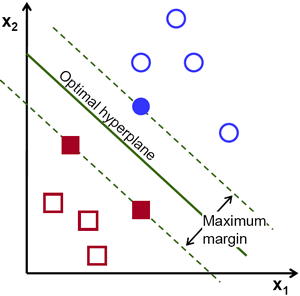
\includegraphics[keepaspectratio,scale=2]{SVM.png} \\ \vspace{5px}
				\Tiny{Image from \url{http://docs.opencv.org/doc/tutorials/ml/introduction_to_svm/introduction_to_svm.html}}
			\end{figure}
			
			\column{.5\textwidth}
			\begin{itemize}
				\item Solid Figures are support vectors.
				\item Due to the maximized margin, unseen figures can be closer to the line than the support vectors and still be correctly classified.
				\item It is easy to see how new points are classified.
			\end{itemize}
		\end{columns}
	}
	
	\subsection{Neural Network}
	\subsubsection{Overview}
	\frame{ \frametitle{Neural Networks}
		\begin{itemize}
			\item Inspired by biological neurons.
			\item Neurons maintain a weighted sum of their inputs. The result of this sum is passed into a function and output. (A step function produces on/off signals while a Sigmoid will produce continues levels of activation.)
			\item The network can be trained by adjusting the weights of the inputs to each neuron.
			\item In a feed-forward network, the backwards propagation algorithm accomplishes this.
			\item Networks with multiple layers can classify various types of non-linearly separable data.
		\end{itemize}
	}
	
	\subsubsection{Structure and Classification}
	\frame{ \frametitle{An Artificial Neuron}
		\begin{figure}
			\centering
			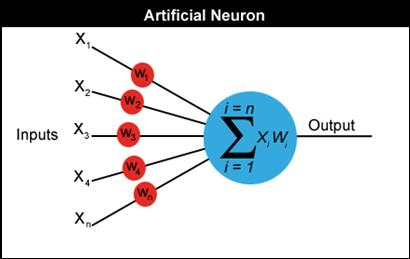
\includegraphics[keepaspectratio,scale=.9]{NN_1.jpg} \\
			\Tiny{Image from \url{http://www.ai-junkie.com/ann/evolved/nnt1.html}}
		\end{figure}
	}
	
	\frame{ \frametitle{Neural Network Classification}
		\begin{columns}[t]
			\column{.5\textwidth}
			\begin{figure}
				\centering
				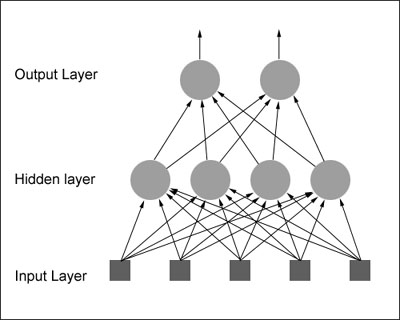
\includegraphics[keepaspectratio,scale=0.4]{NN_2.jpg} \\ \vspace{5px}
				\Tiny{Image from \url{http://www.ai-junkie.com/ann/evolved/nnt1.html}}
			\end{figure}
			
			\column{.5\textwidth}
			\begin{itemize}
				\item Information is fed into the input layer.
				\item The outputs of the neurons in the output layer represent classifications.
				\item Hidden layers perform intermediary manipulations of signals. More hidden layers can be added as needed.
			\end{itemize}
		\end{columns}
	}
	
	\subsection{K-Nearest Neighbor (KNN)}
	\subsubsection{Overview}
	\frame{ \frametitle{K-Nearest Neighbor}
		\begin{itemize}
			\item Assumes that data vectors lie in a metric space.
			\item Training is simple. KNN stores all of the training data points with no computation. (KNN is lazy.) 
			\item Classification is also simple. To classify point \(x\), find the k points in the training data closest to \(x\). Classify \(x\) as the majority vote its k-nearest neighbors.
			\item Can also weight votes based on the distance of the the neighbors.
			\item KNN suffers from the curse of dimensionality. (In high dimensions points start to become equidistant. This means metrics such as Euclidean distance become unhelpful.)
		\end{itemize}
	}
	
	\subsubsection{Example}
	\frame{ \frametitle{KNN Example}
		\begin{columns}[t]
			\column{.5\textwidth}
			\begin{figure}
				\centering
				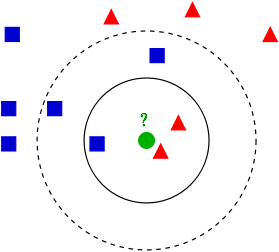
\includegraphics[keepaspectratio,scale=0.5]{KNN.png} \\ \vspace{5px}
				\Tiny{Image from \url{http://en.wikipedia.org/wiki/File:KnnClassification.svg}}
			\end{figure}
			
			\column{.5\textwidth}
			\begin{itemize}
				\item Red and blue points represent training data.
				\item The green point is being classified.
				\item For \(k=3\) the point is classified as red.
				\item For \(k=5\) the point is classified as blue.
				\item Weighting votes by distance may shift favor back to red.
			\end{itemize}
		\end{columns}
	}
	
	\subsection{CART}
	\subsubsection{Overview}
	\frame{ \frametitle{Classification and Regression Tree (CART)}
		\begin{itemize}
			\item Create binary decision trees. Minimize the error in each leaf.
			\item Produces a classification tree for categorical data and a regression tree for numerical data.
			\item Data is recursively split according to rules until a set of stopping rules are met or when no further gain can be made.
			\item Can also split data as much as possible and the prune.
			\item Each internal node is a decision.
			\item Each leaf is a classification, which classifies according to majority vote of training data that follows that tree path.
		\end{itemize}
	}
	
	\subsubsection{Example}
	\frame{ \frametitle{CART Example}
		\begin{columns}[t]
			\column{.5\textwidth}
			\begin{figure}
				\centering
				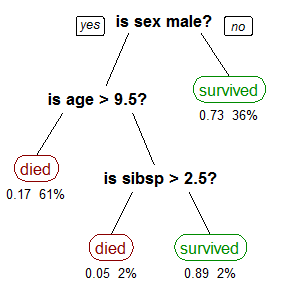
\includegraphics[keepaspectratio,scale=0.5]{CART.png} \\ \vspace{5px}
				\Tiny{Image from \url{http://en.wikipedia.org/wiki/File:CART_tree_titanic_survivors.png}}
			\end{figure}
			
			\column{.5\textwidth}
			\begin{itemize}
				\item CART tree for classifying survival of passengers on the Titanic.
				\item Sibsp is number of spouses and siblings aboard the ship.
				\item Tree also shows probability of survival and percentage of observations.
				\item To classify unseen data point simply follow the tree until a leaf node is met.
			\end{itemize}
		\end{columns}
	}
	
	
	
	% Multivariate stochastic time series T with attributes A1, A2, .. AN, class value C
	% Unique challenges with time series, particularly with validation
	% We have to split the series up into T[1:i], train on that data to create a model,
	%   then using that model, predict T[i+1].
	% We can't do k-fold cross-validation (explain why).
	% Since the time series is stochastic, to some extent the attribute and class values
	%   for this iteration T[i] will depend on values of the previous iterations T[1:i-1].
	% Our conjecture is that adding derived attributes D1, D2, .. DM which are based on
	% values of attributes for previous iterations will improve classification accuracy
	% because they add information which has predictive power.
	% We test hypotheses H1, H2, H3 .. against H0, which is the classication task done
	% with the raw data set (only native attributes).
	% Hypotheses H1, H2, H3 .. consist of computing derived attributes D1, D2, .. DM,
	% then running the new data set through the same classifiers to observe the difference
	% in classifier accuracy (and variance accounted for in the principal components due
	% to the derived attributes).
	\section{Experimental Design}


	% We use the classifier functions in R
	% The major part of our implementation is computing the derived attributes
	% and processing the data set for testing and validation
	\section{Implementation}
	

	% Table: data sets vs. models vs. accuracies given different hypotheses H1, H2, .. H0.
	% Graph of the same.
	\section{Experimental Results}
	

	
\end{document}
